\documentclass[landscape]{article}
\usepackage[a4paper, top=0.5cm, bottom=0.5cm, left=0.5cm, right=0.5cm]{geometry}

\usepackage[utf8]{inputenc}
\usepackage{amsmath, amsfonts, amssymb}
\usepackage{multicol}
\usepackage{graphicx}
\usepackage{blindtext}
\usepackage{paralist}
\usepackage[boxed, vlined]{algorithm2e}
\usepackage{booktabs}

\setlength\parindent{0ex}
\setlength{\columnsep}{10mm}

\newcommand{\vmspace}{\vspace{-7pt}}
\newcommand{\vamspace}{\vspace{-3pt}}
\newcommand{\vpspace}{\vspace{5pt}}
\newcommand{\vtspace}{\vspace{-10pt}}

\begin{document}

\pagestyle{empty}
\raggedright
\setlength{\columnsep}{2mm}
\setlength{\columnseprule}{0.1mm}
\renewcommand{\labelitemi}{--}

\begin{multicols}{3}

%\title{\textbf{Autonomous Mobile Robots}}
%\author{Fabian Bl\"ochliger}
%\date{Spring Semester 2016}
%\maketitle

\begin{tabular}{|c|}\hline
  \\[-8pt]
  \LARGE \textbf{Autonomous Mobile Robots}\\[6pt]
  \large Fabian Bl\"ochliger\\[6pt]
  \large \textit{Spring Semester 2016}\\\hline
\end{tabular}

\vtspace

\section{Introduction and Motivation}

\vmspace

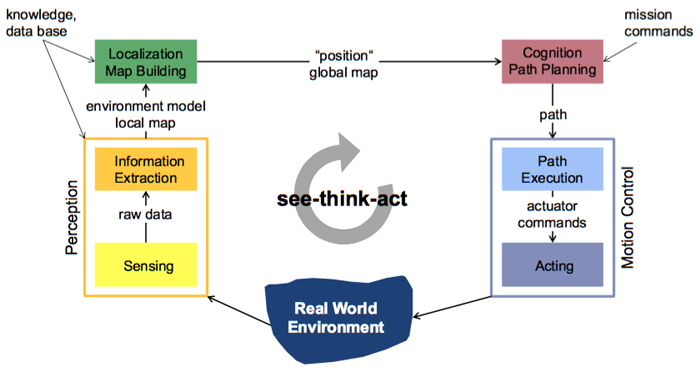
\includegraphics[width=\columnwidth]{img/1_SeeThinkAct.png}

\vspace{-12pt}

\section{Locomotion Concepts}

\vmspace

\begin{minipage}{\columnwidth}
  Express point $P$ which is given w.r.t body frame $B$ in inertial frame $I$:
  \vmspace
  \vmspace
  \begin{center}
  ${}_I\mathbf{r}_{OP} = {}_I\mathbf{r}_{OB} +
  \mathbf{R}_{IB}\;{}_B\mathbf{r}_{BP}$.
  \end{center}
\end{minipage}

\vpspace

\begin{minipage}{\columnwidth}
  Equivalent \textbf{homogeneous transformation} description:
  \vmspace
  \begin{center}
    $\left[\begin{matrix}
      {}_I\mathbf{r}_{OP} \\
      1
    \end{matrix}\right]
    =
    \left[\begin{matrix}
      \mathbf{R}_{IB} & {}_I\mathbf{r}_{OB} \\
      0 & 1
    \end{matrix}\right]
    \left[\begin{matrix}
      {}_B\mathbf{r}_{BP} \\
      1
    \end{matrix}\right]
    =
    \mathbf{H}_{IB}\cdot{}_B\tilde{\mathbf r}_{BP}.
    $
  \end{center}
\end{minipage}

\vpspace

\begin{minipage}{\columnwidth}
  \textbf{Velocity} of rigid body point $P$:
  \vmspace
  \begin{center}
    ${}_I \mathbf v_P = {}_I \mathbf{\dot r}_{OP} = \mathbf{\dot r}_{OB} +
    {}_I\mathbf{\omega}_{IB} \times {}_I\mathbf r_{BP}.$
  \end{center}
\end{minipage}

\vpspace

\begin{minipage}{\columnwidth}
  Differentiation in moving frame (\textbf{Coriolis equation}):
  \vmspace
  \begin{center}
    ${}_B\mathbf v_P = {}_B\left[\mathbf{\dot r}_{OP}\right] = \dfrac{\mathrm
    d\, {}_B\mathbf r_{OP}}{\mathrm d \,t} + {}_B\omega_{IB} \times {}_B\mathbf
    r_{OP}$
  \end{center}
\end{minipage}

\vpspace

\begin{minipage}{\columnwidth}
  Basic rotation matrices $\mathbf R_x(\bullet)$, $\mathbf R_y(\bullet)$, $\mathbf
  R_z(\bullet)$:
  \vmspace
  \begin{center}
    $\left[\begin{matrix}
      1 & 0 & 0 \\
      0 & \cos & -\sin \\
      0 & \sin & \cos
    \end{matrix}\right],\;
    \left[\begin{matrix}
      \cos & 0 & \sin \\
      0 & 1 & 0 \\
      -\sin & 0 & \cos
    \end{matrix}\right],\;
    \left[\begin{matrix}
      \cos & -\sin & 0 \\
      \sin & \cos & 0 \\
      0 & 0 & 1
    \end{matrix}\right].$
  \end{center}
\end{minipage}

\vpspace

\begin{minipage}{\columnwidth}
  \textbf{Jacobian} (partial derivative of position vector $\mathbf{r}(\mathbf
  q)$ w.r.t. \textbf{generalized coordinate} vector $\mathbf{q}$):
  \vmspace
  \begin{center}
    $
    \mathbf J
    =
    \dfrac{\partial \mathbf{r}(\mathbf q)}{\partial \mathbf q}
    =
    \left[
    \begin{matrix}
      \frac{\partial r_1}{\partial q_1} & \cdots & \frac{\partial r_1}{\partial
      q_n} \\
      \vdots & \ddots & \vdots \\
      \frac{\partial r_m}{\partial q_1} & \cdots & \frac{\partial r_m}{\partial
      q_n} \\
    \end{matrix}
    \right]
    $.
  \end{center}
\end{minipage}

\vpspace

\begin{minipage}{\columnwidth}
  Left/right pseudoinverse for $m \times n$ matrix $\mathbf{J}$ to solve
  $\mathbf r_F = \mathbf J_F \mathbf q$ for $\mathbf q$:
  \vmspace
  \begin{center}
    $\mathbf{J}^+=
    \begin{cases}
      (\mathbf{J}^\intercal \mathbf J)^{-1} \mathbf J^\intercal, & m>n\;\;
      \text{(overdetermined)},\\
      \mathbf J^\intercal (\mathbf{J} \mathbf J^\intercal)^{-1}, & m<n\;\;
      \text{(underdetermined).}
    \end{cases}$
  \end{center}
\end{minipage}

\vpspace

\begin{minipage}{\columnwidth}
  Iterative approach for \textbf{inverse kinematics} of robotic manipulator to
  find generalized coordinates for end-effector position $\mathbf r^\text{goal}$
  (Newton's method):

  \vamspace

  \begin{algorithm}[H]
    \DontPrintSemicolon
    $\mathbf q = \mathbf q^0,\;\mathbf r = \mathbf r(\mathbf q)$\;
    \While{$\| \mathbf r - \mathbf r^\mathrm{goal} \| > \mathrm{threshold}$}
    {
    $\mathbf q = \mathbf q + \mathbf J^+(\mathbf q) \cdot (\mathbf r^\text{goal}
    - \mathbf r),\;\;
    \mathbf r = \mathbf r ( \mathbf q )$\;
    }
  \end{algorithm}
\end{minipage}

\vpspace

\begin{minipage}{\columnwidth}
  Inverse \textbf{differential kinematics} (get desired end-effector velocity
  $\mathbf{\dot{r}_F}$):
  \vmspace
  \begin{center}
    $\mathbf{\dot r}_F = \mathbf J_F \mathbf{\dot q}$
    $\;\;\rightarrow\;\;$
    $\mathbf{\dot q} = \mathbf J_F^+ \mathbf r_F.$
  \end{center}
\end{minipage}

% TODO
% - Check column-rank / row-rank deficiency.

\vtspace

\section{Mobile Robot Kinematics}

\vmspace

\begin{minipage}{\columnwidth}
  \textbf{General wheel equation} ($\mathbf v_{IR}, \omega_{IR}$: linear /
  angular robot velocity, $\omega_{RS}$: steer rate, $\mathbf r_{SW}$: wheel
  offset):
  \vmspace
  \begin{center}
    $\mathbf v_{IW} = \mathbf v_{IR} + \omega_{IR} \times [\mathbf r_{RS} +
    \mathbf r_{SW}] +
    \omega_{RS} \times \mathbf r_{SW}.$
  \end{center}
\end{minipage}

\vpspace

\begin{minipage}{\columnwidth}
  \textbf{Standard wheel equation} (no wheel offset $\mathbf r_{SW}$):
  \vmspace
  \begin{center}
    $\mathbf v_{IW} = \mathbf v_{IR} + \omega_{IR} \times \mathbf r_{RS}.$
  \end{center}
\end{minipage}

\vspace{3pt}

\begin{minipage}{\columnwidth}
  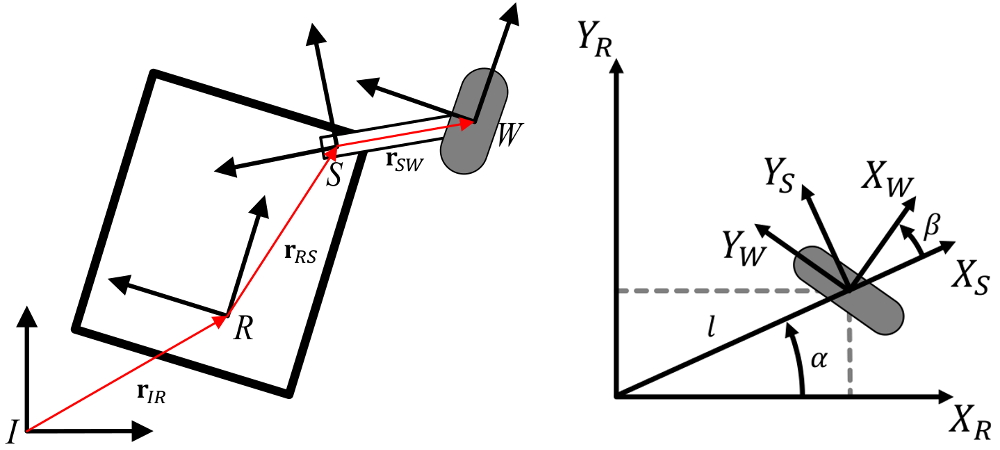
\includegraphics[width=\columnwidth]{img/3_WheelEquations.png}
\end{minipage}

\vspace{5pt}

\begin{minipage}{\columnwidth}
  Rolling constraint (${}_W\mathbf v_{IW} = [0, -r\dot\varphi, 0]^\intercal$):
  \vmspace
  \begin{center}
    $\left[\begin{matrix}
      \sin(\alpha + \beta) & -\cos(\alpha + \beta) & (-l) \cos(\beta)
    \end{matrix}\right]
    R(\theta)\dot\xi_I
    =
    r \dot \varphi.$
  \end{center}
\end{minipage}

\begin{minipage}{\columnwidth}
  No-sliding constraint:
  \vmspace
  \begin{center}
    $\left[\begin{matrix}
      \cos(\alpha + \beta) & \sin(\alpha + \beta) & l \sin(\beta)
    \end{matrix}\right]
    R(\theta)\dot\xi_I
    =
    0.$
  \end{center}
\end{minipage}

\begin{minipage}{\columnwidth}
  Robot state:
    $\xi_I
    =
    \left[\begin{matrix}
      x & y & \theta
    \end{matrix}\right]^\intercal,
    \;\;
    \dot\xi_R = R(\theta)\dot\xi_I,
    \;\;
    R(\theta) = \mathbf R_z^\intercal(\theta).$
\end{minipage}

\vpspace

\begin{minipage}{\columnwidth}
  Stacked equations of motion for a $(N_f+N_s)$-wheeled robot:
  \vmspace
  \begin{center}
    $\begin{matrix}
      \text{\textbf{(rolling)}}\;\;\;\;\;\; \\
      \text{\textbf{(no-sliding)}}
    \end{matrix}\;\;
    \left[\begin{matrix}
      J_1(\beta_s) \\
      C_1(\beta_s)
    \end{matrix}\right]
    R(\theta)\dot\xi_I
    =
    \left[\begin{matrix}
      J_2 \\
      0
    \end{matrix}\right]
    \dot\varphi,\;\;\;\;
    \dot\varphi
    =
    \left[\begin{matrix}
      \dot\varphi_1..\dot\varphi_N
    \end{matrix}\right],$
  \end{center}
\end{minipage}

\begin{minipage}{\columnwidth}
  with
  \vmspace
  \begin{center}
    $J_1(\beta_s)
    =
    \left[\begin{matrix}
      J_{1f} \\
      J_{1s}(\beta_s)
    \end{matrix}\right],
    J_2
    =
    \mathrm{diag}(r_1..r_N),
    C_1(\beta_s)
    =
    \left[\begin{matrix}
      C_{1f} \\
      C_{1s}(\beta_s)
    \end{matrix}\right].$
  \end{center}
\end{minipage}

\vpspace

\begin{minipage}{\columnwidth}
  A robot's \textbf{degree of maneuverability} $\varphi_M$ is
  \vmspace
  \begin{center}
    $\delta_M = \delta_m + \delta_s$,
  \end{center}
  \vmspace
  which is the sum of its \textbf{degree of mobility} $\varphi_m$ and its
  \textbf{degree of steerability} $\varphi_s$:
  \vmspace
  \begin{center}
    $\delta_m=\mathrm{dim}\,\mathrm{N}\left[C_1(\beta_s)\right] = 3 -
    \mathrm{rank}\left[C_1(\beta_s)\right],\;
    \varphi_s = \mathrm{rank}\left[C_{1s}(\beta_s)\right].$
  \end{center}
\end{minipage}

\vpspace

\begin{minipage}{\columnwidth}
  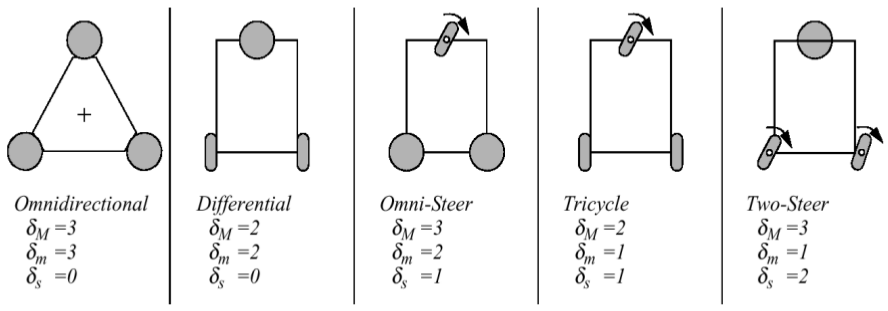
\includegraphics[width=\columnwidth]{img/3_WheelTypes.png}
\end{minipage}

\begin{minipage}{\columnwidth}
  Forward/inverse kinematics of a \textbf{differential drive robot}:
  \vmspace
  \begin{center}
    $
    \left[
    \begin{matrix}
      \dot x \\
      \dot y \\
      \dot \theta
    \end{matrix}
    \right]_R
    =
    \left[
    \begin{matrix}
      \frac{r}{2} & \frac{r}{2} \\
      0 & 0 \\
      \frac{r}{2b} & -\frac{r}{2b}
    \end{matrix}
    \right]
    \left[
    \begin{matrix}
      \dot \varphi_r \\
      \dot \varphi_l
    \end{matrix}
    \right]
    \;\; / \;\;
    \left[
    \begin{matrix}
      \dot \varphi_r \\
      \dot \varphi_l
    \end{matrix}
    \right]
    =
    \left[
    \begin{matrix}
      \frac{1}{r} & 0 & \frac{b}{r} \\
      \frac{1}{r} & 0 & -\frac{b}{r}
    \end{matrix}
    \right]
    \left[
    \begin{matrix}
      \dot x \\
      \dot y \\
      \dot \theta
    \end{matrix}
    \right]_R
    $.
  \end{center}
\end{minipage}

% TODO
% Add if more space:
% - differential kinematics
% - general wheel equation
% - kinematics of differential drive robot
% - wheel equation of swedish/castor wheel

\vtspace

\section{Perception I}
\vmspace

\begin{minipage}{\columnwidth}
  \begin{center}
    \begin{tabular}{lll}\toprule
      \textbf{Sensor Type} & \textbf{System} & \textbf{Class} \\\hline
      Tactile & Bumpers & EC, P \\
      Wheel/motor & Brush encoders & PC, P \\
      & Optical encoders & PC, A \\
      Heading & Compass & EC, P \\
      & Gyroscope & PC, P \\
      & Inclinometer & EC, A/P \\
      Acceleration & Accelerometer & PC, P \\
      Beacons & GPS & EC, A \\
              & Radio, ultrasonic, & EC, A \\
              & Reflective Beacons \\
      Motion/speed & Doppler: radar/sound & EC, A \\
      Range & Ultrasound, laser, & EC, A \\
            & struct. light, ToF \\
      Vision & CCD/CMOS & EC, P \\
      \bottomrule
      \\[-10pt]
      \multicolumn{3}{l}{(PC = \textbf{proprioceptive}, EC =
      \textbf{exteroceptive},} \\
      \multicolumn{3}{l}{A = active, P = passive)}
    \end{tabular}
  \end{center}
\end{minipage}

\vpspace

\begin{minipage}{\columnwidth}
  \textbf{Range sensors}: Traveled distance $d$ of a sound or electromagnetic
  wave after a \textbf{time of flight} $t$ is given by
  \vmspace
  \begin{center}
    $d=ct,\;\;\; c = 0.3\,\mathrm m / \mathrm{ms}\,\text{(sound)} \; / \;
    0.3\,\mathrm m / \mathrm{ns}\,\text{(light)}.$
  \end{center}
\end{minipage}

\vpspace

\begin{minipage}{\columnwidth}
  The \textbf{mean/expectation value} $\mathrm{E}[x] = \mu$ and the
  \textbf{variance} $\mathrm{Var}[x] = \sigma^2$ of a \textbf{continuous random
  variable} $x$ with \textbf{probability density function (PDF)} $p(x)$ are
  computed as
  \vmspace
  \begin{center}
    $\mu = \int_{-\infty}^{\infty}xp(x)\mathrm dx,\;\;
    \sigma^2 = \int_{-\infty}^{\infty} = (x - \mu)^2 p(x)
    \mathrm dx.$
  \end{center}
\end{minipage}

\vpspace

\begin{minipage}{\columnwidth}
  The PDF for a one-dimensional \textbf{Gaussian distribution}:
  \vmspace
  \begin{center}
    $p(x)
    =
    \mathcal N (\mu, \sigma^2)
    =
    \dfrac{1}{\sigma \sqrt{2\pi}}\,\mathrm{exp}\left[-\dfrac{(x -
    \mu)^2}{2\sigma^2}\right].$
  \end{center}
\end{minipage}

\vpspace

\begin{minipage}{\columnwidth}
  The \textbf{error propagation law} describes the mapping from input covariance
  $C_X$ to output covariance $C_Y$ using the Jacobian $F_X$ of the mapping
  function $f(\bullet): \mathbb{R}^n \rightarrow \mathbb{R}^m$ w.r.t. $X$:
  \vmspace
  \begin{center}
    $C_Y=F_XC_XF_X^\intercal\;\;\text{(linear approximation)}.$
  \end{center}
\end{minipage}

% TODO:
% - Error propagation law
% - Phase shift of laser rangefinder
% - Intro to Computer Vision / Human Vision

\vtspace

\section{Perception II}

\vmspace

\begin{minipage}{\columnwidth}
  \textbf{Thin lens equation:} Voxel at depth $z$ will be \textbf{focused} on
  the \textbf{focal plane} at distance $e$ behind the lens for a camera with
  \textbf{focal length} $f$. If the \textbf{image plane} lies at $e \pm \delta$,
  the voxel image will be a \textbf{blur circle} of radius $R$:
  \vmspace
  \begin{center}
    $\dfrac{1}{f} = \dfrac{1}{z} + \dfrac{1}{e},\;\; R = \dfrac{L \delta}{2e}
    \;\;
    (L:\;\text{diameter of lens/aperture}).$
  \end{center}
\end{minipage}

\vpspace

\begin{minipage}{\columnwidth}
  \textbf{Pinhole approximation:} $z \gg f$, therefore $e \approx f$ (lens is
  approximated as pinhole at distance $f$ from image plane).
\end{minipage}

\vpspace

\begin{minipage}{\columnwidth}
  \textbf{Perspective projection:} A 3D-point $P_C=[X_C,Y_C,Z_C]^\intercal$ (in
  camera frame $C$) projects
  onto the image location $[u,v]^\intercal$ as
  \vmspace
  \begin{center}
    $\left[\begin{matrix}
      u \\
      v
    \end{matrix}\right]
    =
    \left[\begin{matrix}
      \alpha_u\,X_C/Z_C + u_0 \\
      \alpha_v\,Y_C/Z_C + v_0
    \end{matrix}\right]\;\;/\;\;
    \lambda
    \left[\begin{matrix}
      u \\
      v \\
      1
    \end{matrix}\right]
    =
    \underbrace{\left[\begin{matrix}
      \alpha_u & 0   & u_0 \\
      0   & \alpha_v & v_0 \\
      0   & 0   & 1
    \end{matrix}\right]}_{\text{calibr. matrix}\; K}
    \left[\begin{matrix}
      X_C \\
      Y_C \\
      Z_C
    \end{matrix}\right],
    $
  \end{center}
  \vmspace with $[\alpha_u, \alpha_v] = f [k_u,k_v]$, using the inverse of the
  effective pixel size $k_u$ ($k_v$) in $[\mathrm{pixel}/\mathrm{m}]$ and the
  pixel coordinates of the \textbf{optical center} $[u_0,v_0]^\intercal$. $K$
  contains the \textbf{intrinsic parameters}.
\end{minipage}

\vpspace

\begin{minipage}{\columnwidth}
  \textbf{Radial distortion} model:
  \vmspace
  \begin{center}
    $
    \left[\begin{matrix}
      u_{\mathrm d} \\
      v_{\mathrm d}
    \end{matrix}\right]
    =
    (1 + k_1 r^2)
    \left[\begin{matrix}
      u - u_0 \\
      v - v_0
    \end{matrix}\right]
    +
    \left[\begin{matrix}
      u_0 \\
      v_0
    \end{matrix}\right],\;\;
    r^2 = (u - u_0)^2 + (v - v_0)^2.
    $
  \end{center}
\end{minipage}

\vpspace

\begin{minipage}{\columnwidth}
  For a \textbf{general perspective projection}, $P_W$ is given w.r.t. world
  frame $W$ and the transform from $W$ to $C$ is described by the
  \textbf{extrinsic parameters} $[R|T]$.
  \vmspace
  \begin{center}
    $
    \lambda
    \left[\begin{matrix}
      u \\
      v \\
      1
    \end{matrix}\right]
    =
    K\left(R
    \left[\begin{matrix}
      X_W \\
      Y_W \\
      Z_W
    \end{matrix}\right]
    + T\right)
    =
    \underbrace{
    K[R|T]
    }_{\substack{\text{camera} \\ \text{matrix}\;P}}
    \left[\begin{matrix}
      X_W \\
      Y_W \\
      Z_W \\
      1
    \end{matrix}\right].
    $
  \end{center}
\end{minipage}

% TODO: Check R, T.

\vpspace

\begin{minipage}{\columnwidth}
  Basic stereo camera setup with \textbf{baseline} $b$ and focal length $f$, the
  depth $Z$ for a point at left/right coordinate $[u_l,u_r]$ is
  \vmspace
  \begin{center}
    $Z = bf/d,\;\;
    d = u_l - u_r\;(\text{disparity}).$
  \end{center}
\end{minipage}
\vpspace

\begin{minipage}{\columnwidth}
  Cross-product written with skew-symmetric matrix:
  \vmspace
  \begin{center}
    $
    \mathbf a \times \mathbf b = [\mathbf a_\times ] \mathbf b
    =
    \left[
    \begin{matrix}
      0 & -a_z & a_y \\
      a_z & 0 & - a_x \\
      -a_y & a_x & 0
    \end{matrix}
    \right]
    \left[
    \begin{matrix}
      b_x \\
      b_y \\
      b_z
    \end{matrix}
    \right].
    $
  \end{center}
\end{minipage}

\vpspace

\begin{minipage}{\columnwidth}
  \textbf{Epipolar constraint} ($p_1, p_2$: normalized, homogeneous):
  \vmspace
  \begin{center}
    $p_2^\intercal E p_1 = 0,\;\; E = [T_\times]R\;\text{(essential matrix)}.$
  \end{center}
  \vspace{-18pt}
  \begin{center}
    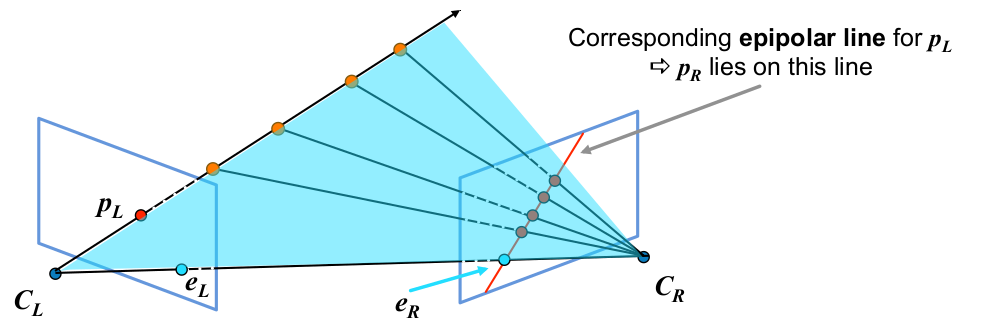
\includegraphics[width=0.9\columnwidth]{img/5_EpipolarConstraint.png}
  \end{center}
\end{minipage}

\vfill

\vtspace

\section{Perception III}

\vmspace

\begin{minipage}{\columnwidth}
  \textbf{Correlation} with a filter/kernel/mask $F$ of size $(2N+1)$ is
  \vmspace
  \begin{center}
    $J(x) = F \circ I(x) = \sum_{i=-N}^N F(i) I(x + i)$,
  \end{center}
\end{minipage}

\begin{minipage}{\columnwidth}
  \textbf{Convolution} is correlation with a flipped filter/image:
  \vmspace
  \begin{center}
    $J(x) = F \ast I(x) = \sum_{i=-N}^N F(i) I(x - i)$.
  \end{center}
  \vmspace
  In contrast to correlation, convolution is associative.
\end{minipage}

\vpspace

\begin{minipage}{\columnwidth}
  \textbf{Linear filters} replace every pixel by a linear combination of its
  neighbors. \textbf{Shift-invariant filters} perform the same operation on
  every point of the image.
\end{minipage}

\vpspace

\begin{minipage}{\columnwidth}
  The \textbf{2D Gaussian kernel} is a \textbf{separable} filter (width
  $\sigma$):
  \vmspace
  \begin{center}
    $
    G_\sigma = (x, y) = \frac{1}{2\pi\sigma^2}
    \,\mathrm e^{-\frac{x^2 + y^2}{2 \sigma ^2}}
    =
    \underbrace{\tfrac{1}{\sigma \sqrt{2\pi}}
    \,\mathrm e^{-\frac{-x^2}{2\sigma^2}}}_{g_\sigma(x)}
    \cdot
    \underbrace{\tfrac{1}{\sigma \sqrt{2\pi}}
    \,\mathrm e^{-\frac{-y^2}{2\sigma^2}}}_{g_\sigma(y)}.
    $
  \end{center}
\end{minipage}

\vspace{3pt}

\begin{minipage}{\columnwidth}
  \textbf{Laplacian of Gaussian} (second derivative operator):
  \vmspace
  \begin{center}
    $\mathrm{LoG} = \nabla^2 G_\sigma(x, y) = \frac{\partial^2 G_\sigma(x,
    y)}{\partial x^2} + \frac{\partial^2 G_\sigma(x, y)}{\partial y^2}.
    $
  \end{center}
\end{minipage}

\vpspace

\begin{minipage}{\columnwidth}
  \textbf{Difference of Gaussian} is an approximation of LoG:
  \vmspace
  \begin{center}
    $\mathrm{DoG} = G_{k\sigma}(x, y) - G_\sigma(x, y).
    $
  \end{center}
\end{minipage}

\vpspace

\begin{minipage}{\columnwidth}
  \textbf{Template matching} using \textbf{sum of squared differences}:
  \vmspace
  \vspace{-3pt}
  \begin{equation*}
    \begin{split}
      \mathrm{SSD}(x) &= \mathsmaller\sum\nolimits_{i=-N}^N \left[ F(i) - I(x+i)
      \right]^2,\\
      &= \mathsmaller\sum \left[ F(i) \right]^2 +
      \mathsmaller\sum \left[ I(x+i) \right]^2 -
      2 \mathsmaller\sum \left[ F(i) I(x+i) \right].
    \end{split}
  \end{equation*}
\end{minipage}

\vpspace

\begin{minipage}{\columnwidth}
  \textbf{Zero-mean normalized cross correlation (ZNCC)}: Invariant to local
  average intensity. Maximize:
  \vmspace
  \begin{center}
  $
  \mathrm{ZNCC}(x) = \dfrac{\sum_i
    \left[F(i)- \mu_F\right] \left[I(x + i) - \mu_{I_x} \right]}
  {
    \sqrt{\sum_i \left[F(i) - \mu_F\right]^2}
    \sqrt{\sum_i \left[I(x+i) - \mu_{I_x}\right]^2}
  },
    $\\[3pt]
  $
    \mu_F = \frac{\sum_i F(i)}{2N + 1},\;\;
    \mu_{I_x} = \frac{\sum_i I(x+i)}{2N + 1},\;\;
    i=-N..N.
  $
  \end{center}
\end{minipage}

\vpspace

\begin{minipage}{\columnwidth}
  \textbf{Roberts/Prewitt/Sobel masks} (approx. derivatives):
  \vmspace
  \begin{center}
    $I_x =$
    \setlength\tabcolsep{1.2pt}
    \begin{tabular}{|c|c|c|}\hline
      0 & -1 \\\hline
      1 & 0 \\\hline
    \end{tabular} /
    \begin{tabular}{|c|c|c|}\hline
      -1 & 0 & 1 \\\hline
      -1 & 0 & 1 \\\hline
      -1 & 0 & 1 \\\hline
    \end{tabular} /
    \begin{tabular}{|c|c|c|}\hline
      -1 & 0 & 1 \\\hline
      -2 & 0 & 2 \\\hline
      -1 & 0 & 1 \\\hline
    \end{tabular} ,
    $\;I_y =$
    \begin{tabular}{|c|c|c|}\hline
      -1 & 0 \\\hline
      0 & 1 \\\hline
    \end{tabular} /
    \begin{tabular}{|c|c|c|}\hline
      -1 & -1 & -1 \\\hline
      0 & 0 & 0 \\\hline
      1 & 1 & 1 \\\hline
    \end{tabular} /
    \begin{tabular}{|c|c|c|}\hline
      -1 & -2 & -1 \\\hline
      0 & 0 & 0 \\\hline
      1 & 2 & 1 \\\hline
    \end{tabular} .
  \end{center}
\end{minipage}

\vpspace

\begin{minipage}{\columnwidth}
  The \textbf{second order matrix} used by the \textbf{Harris corner detector}
  (image patch size $P$):
  \vmspace
  \begin{center}
    $M = \sum\limits_{x, y \in P}
    \left[
    \begin{matrix}
      I_x^2 & I_x I_y \\
      I_x I_y & I_y^2
    \end{matrix}
    \right],\;
    \mathrm{SSD}(\Delta x, \Delta y)
    \approx
    \left[
    \begin{matrix}
      \Delta x\,\Delta y
    \end{matrix}
    \right]
    M
    \left[
    \begin{matrix}
      \Delta x \\
      \Delta y
    \end{matrix}
    \right].
    $
  \end{center}
  \vmspace
  Corners: Local maxima in the \textbf{cornerness function}
  \vmspace
  \begin{center}
    $C = \lambda_1\lambda_2 - \kappa (\lambda_1 + \lambda_2)^2
    = \mathrm{det}\,M - \kappa\,\mathrm{trace}^2 M.$
  \end{center}
\end{minipage}

\vpspace

\begin{minipage}{\columnwidth}
  Main \textbf{SIFT} stages: \\[-2pt]
  \begin{minipage}{\columnwidth}
    \begin{minipage}{0.5\columnwidth}
      1. Extract keypoints + scale. \\
      2. Assign keypoint orientation. \\
      3. Generate descriptor ($4\cdot 4\cdot 8$). \\
      $[$4. Matching ($L_2$ distance).$]$
    \end{minipage}
    \begin{minipage}{0.49\columnwidth}
      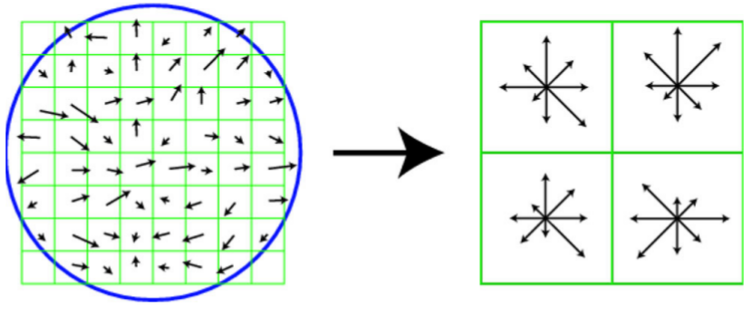
\includegraphics[width=\columnwidth]{img/6_SIFT.png}
    \end{minipage}
  \end{minipage}
\end{minipage}

\section{Perception IV}

\vmspace

\vspace{-5pt}
\begin{center}
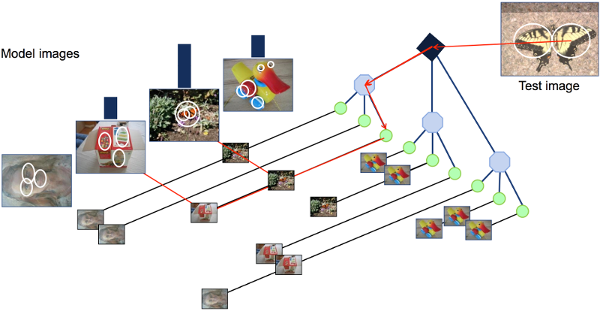
\includegraphics[width=0.85\columnwidth]{img/7_VocabularyTree.png}
\end{center}
\vspace{-10pt}

\begin{minipage}{\columnwidth}
  Vector quantization by \textbf{k-means clustering}, minimizes squared
  Euclidean distance between points and their nearest cluster-centers:

  \vamspace

  \begin{algorithm}[H]
    \DontPrintSemicolon
    randomly initialize $k$ cluster centers\;
    \While{not converged}
    {
      assign each vector to nearest center\;
      re-compute cluster centers\;
    }
  \end{algorithm}
\end{minipage}

\begin{minipage}{\columnwidth}
  \textit{Line extraction algorithms:}\\
  A1) \textbf{Split-and-merge:}
  \begin{compactenum}
  \item Fit line through point set, find most distant point $P$.
  \item If $d_P > \mathrm{threshold}$, split set at $P$. Repeat for all sets.
  \item If two consecutive segments are collinear enough, merge.
  \end{compactenum}
\end{minipage}

\vpspace

\begin{minipage}{\columnwidth}
  A2) \textbf{Line regression:}
  \begin{compactenum}
  \item Initialize sliding window size $N_f$.
  \item Fit a line to every $N_f$ consecutive points.
  \item Merge overlapping line segments and re-compute line parameters for each
    segment.
  \end{compactenum}
\end{minipage}

\vpspace

\begin{minipage}{\columnwidth}
  A3) \textbf{RANSAC:}
  \begin{compactenum}
  \item Randomly select 2 points and fit a line through them.
  \item Compute distances of all points to this line, select inliers.
  \item Iterate $k$ times. Estimate $k=\log(1-p)/\log(1-w^2)$ ($p$:
    probability of finding set free of outliers, $w$: fraction of inliers).
  \end{compactenum}
\end{minipage}

\vpspace

\begin{minipage}{\columnwidth}
  A4) \textbf{Hough transform:}
  \begin{compactenum}
  \item For each point $(x,y)$, compute $\rho = x\cos\theta + y\sin\theta$ for
    $\theta=[0..180]$. Increment according array entries.
  \item Find local maxima $(\theta,\rho)$.
  \end{compactenum}
  \vmspace
  \begin{center}
    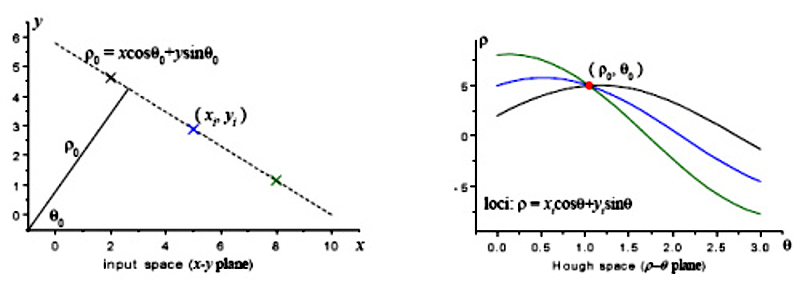
\includegraphics[width=0.9\columnwidth]{img/7_Hough.png}
  \end{center}
\end{minipage}


%  Line extraction using the \textbf{Hough transform}: Map point $(x, y)$ to
%  sinusoid in $(\theta, \rho)$ parameter space according to
%  \vmspace
%  \begin{center}
%    $x \cos \theta + y \sin \theta = \rho.$
%  \end{center}
%  \vspace{-25pt}
%  \begin{center}
%  \end{center}
%\end{minipage}


% TODO:
% -line fitting algorithms

\vfill


\section{Localization I}

\vmspace


\begin{minipage}{\columnwidth}
  \textbf{Sum rule} (1) and \textbf{product rule} (2):
  \vmspace
  \begin{center}
    (1) $p(x) = \sum_y p(x,y),\;\;$
    (2) $p(x, y) = p(y | x) p(x)$.
  \end{center}
\end{minipage}

\vpspace

\begin{minipage}{\columnwidth}
  Combine them to get the \textbf{theorem of total probability}:
  \vmspace
  \begin{center}
    $p(x) = \sum_y p(y | x) p(x).$
  \end{center}
\end{minipage}

\vpspace

\begin{minipage}{\columnwidth}
  Assuming that $p(y) > 0$, \textbf{Bayes' rule} is
  \vmspace
  \begin{center}
    $p(x|y) = \frac{p(y|x)p(x)}{p(y)} = \eta\, p(y|x)p(x),\;\;\;
    \eta = p(y)^{-1}.$
  \end{center}
\end{minipage}

\vpspace

\begin{minipage}{\columnwidth}
  \textbf{Multivariate Gaussian distribution} $\mathcal N(\mu, \Sigma)$ for
  dimension $k$ with (symmetric) covariance matrix $\Sigma$:
  \vmspace
  \begin{center}
    $
    p(x)
    =
    \frac{1}{(2\pi)^{k/2}\,\mathrm{det}(\Sigma)^{1/2}}\,
    \exp\left[
    -\frac{1}{2}(x-\mu)^\intercal \Sigma^{-1} (x-\mu)
    \right].
    $
  \end{center}
\end{minipage}

\vpspace

\begin{minipage}{\columnwidth}
  \textbf{Combination of GRVs:} Let $y=Ax_1 + Bx_2$ be a linear function of
  $x_i=\mathcal N(\mu_i, \Sigma_i)$. Then, $p(y)$ is
  \vmspace
  \begin{center}
    $
    p(y) = \mathcal N (A\mu_1 + B\mu_2,\,
    A\Sigma_1A^\intercal + B\Sigma_2B^\intercal).
    $
  \end{center}
  \vmspace
  If $y=f(x_1,x_2)$ is non-linear, approximate $y$ and $p(y)$ as
  \vmspace
  \begin{center}
    $
    y \approx f(\mu_1, \mu_2) + F_{x_1} (x_1 - \mu_1) + F_{x_2}(x_2 -
    \mu_2),\;\;$\\
    $p(y) \approx \mathcal N(f(\mu_1, \mu_2),\,
    F_{x_1}\Sigma_1{F_{x_1}}^\intercal +
    F_{x_2}\Sigma_2{F_{x_2}}^\intercal).
    $
  \end{center}
\end{minipage}

\vpspace

\begin{minipage}{\columnwidth}
  A robot's \textbf{belief} about its state $x_t$ before/after measurement $z_t$
  is represented as probability distribution:
  \vmspace
  \begin{center}
    $
    \overline{bel}(x_t)
    =
    p(x_t | z_{1 \rightarrow t-1}, u_{1 \rightarrow t}),\;\;
    bel(x_t)
    =
    p(x_t | z_{1 \rightarrow t}, u_{1 \rightarrow t}).
    $
  \end{center}
\end{minipage}

\vpspace

\begin{minipage}{\columnwidth}
  Ingredients of probabilistic \textbf{map-based localization}:
  \begin{compactenum}
  \item The initial probability distribution $bel(x_0)$.
  \item \textit{True} \textbf{map} $M = \{m_0.. m_n\}$ of the environment.
  \item Data: $u_t$ (proprioceptive, control), $z_t$ (exteroceptive).
  \item Probabilistic \textbf{motion model} $p(x_t|u_t, x_{t-1})$, e.g. based on
    noise-free model $x_t = f(x_{t-1}, u_t)$.
  \item Probabilistic \textbf{measurement model} $p(z_t|x_t,M)$, e.g. based on
    noise-free model $z_t = h(x_t, M)$.
  \end{compactenum}
\end{minipage}

\vpspace

\begin{minipage}{\columnwidth}
  Classification of localization problems:
  \begin{compactitem}
  \item \textbf{Position tracking:} $bel(x_0)$ is \textbf{Dirac delta}
    function.
  \item \textbf{Global localization:} Uniform distribution for $bel(x_0))$.
  \item \textbf{Kidnapped robot problem:} Does the robot realize?
  \end{compactitem}
\end{minipage}

\vpspace

\begin{minipage}{\columnwidth}
  \begin{tabular}{p{0.44\columnwidth}p{0.44\columnwidth}}
    Architecture map:\newline

    \vspace{-20pt}

    \begin{center}
      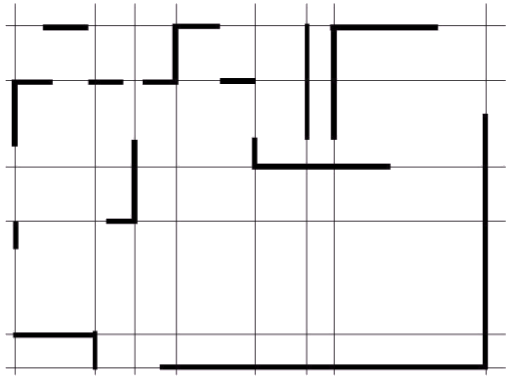
\includegraphics[width=0.28\columnwidth]{img/8_Architecture.png}
    \end{center}
    & Exact cell decomposition:\newline

    \vspace{-20pt}

    \begin{center}
      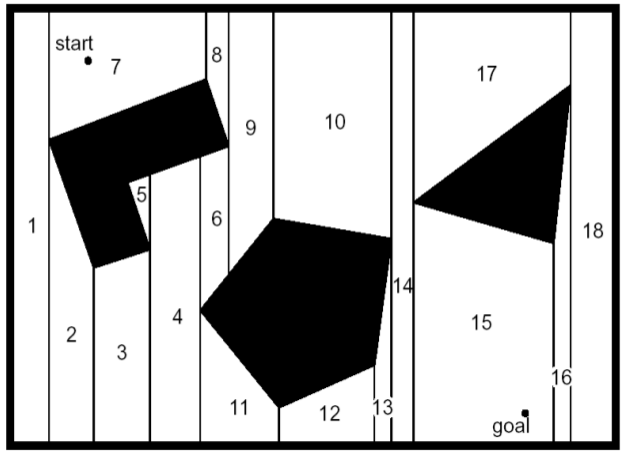
\includegraphics[width=0.29\columnwidth]{img/8_Exact.png}
    \end{center}
    \\[-12pt]
    Approx. decomposition:\newline

    \vspace{-20pt}

    \begin{center}
      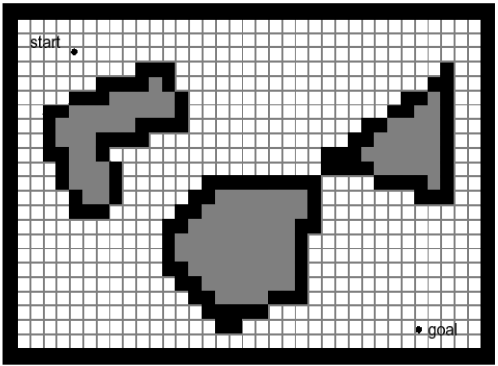
\includegraphics[width=0.29\columnwidth]{img/8_Approx.png}
    \end{center}
    & Topological:\newline

    \vspace{-20pt}

    \begin{center}
      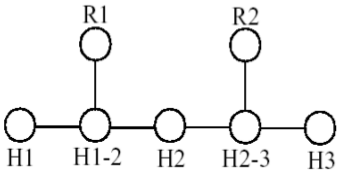
\includegraphics[width=0.38\columnwidth]{img/8_Topological.png}
    \end{center}


    \\[-15pt]
  \end{tabular}
\end{minipage}

% TODO
% - Odometry uncertainty
% - measurement / motion model with uncertainty

\vfill

\vtspace

\section{Localization II}

\vmspace

\begin{minipage}{\columnwidth}
  According to the \textbf{Markov assumption}, the robot's belief state
  $bel(x_t)$ is a function only of robot's previous state $x_{t-1}$ and its most
  recent actions $u_t$ and observations $z_t$:
  \vmspace
  \begin{center}
    $
    p(x_t|x_0, u_0 \cdots u_t, z_0 \cdots z_t)
    =
    p(x_t|x_{t-1}, u_t, z_t).
    $
  \end{center}
\end{minipage}

\vpspace

\begin{minipage}{\columnwidth}
  The general algorithm for \textbf{Markov localization}:

  \vamspace

  \begin{algorithm}[H]
    \DontPrintSemicolon
    \For{\textnormal{\textbf{all}} $x_t$}
    {
    $
    \overline{bel}(x_t)
    =
    \sum_{x_{t-1}} p(x_t|u_t, x_{t-1}) bel(x_{t-1})
    \;\;
    \text{(prediction)}
    $\;
    $
    bel(x_t)
    =
    \eta p(z_t|x_t, M) \overline{bel}(x_t)
    $
    \hspace{29pt}
    $
    \text{(measurement)}
    $\;
    }
  \end{algorithm}
\end{minipage}

\vpspace


\begin{minipage}{\columnwidth}
  \textbf{Kalman filter localization} assumes
  $bel(x_t) = \mathcal N (x_t, P_t).  $\\
  S1) The \textbf{prediction update} is ($Q_t$: covariance of motion model
  noise, $F_{x/u}$: jacobian w.r.t. $x$/$u$):
  \vmspace
  \begin{center}
    $
    \hat x_t = f(x_{t-1}, u_t),\;\;
    \hat P_t = F_x P_{t-1} F_x^\intercal + F_u Q_t F_u^\intercal.
    $
  \end{center}
  \vmspace
  S2) The \textbf{measurement update} consists of four steps:
  \begin{compactenum}
  \item \textit{Observation}: Obtain $z_t^i$ with
    covariance $R_t^i$ ($i=1..n$).
  \item \textit{Measurement prediction}: Predict $\hat z_t^j = h^j(\hat x_t, m^j)$,
    compute its jacobian $H^j$ w.r.t $\hat x_t$.
  \item \textit{Matching step}: Compute the \textbf{innovation}
    (\textbf{covariance})

    \begin{center}
      $
      v_t^{ij}=[z_t^i - z_t^j],\;\;
      \Sigma_{IN_t}^{ij} = H^j \hat P_t {H^j}^\intercal + R_t^i,
      $
    \end{center}

    Find matches with a \textbf{validation gate} $g$, e.g. Mahalanobis distance:
    ${v_t^{ij}}^\intercal (\Sigma_{IN_t}^{ij})^{-1} v_t^{ij} \le g^2$.

  \item \textit{Estimation step}: Stack validated observations into $z_t$, corresponding
    innovations into $v_t$, measurement jacobians into $H_t$ and
    $R_t = \mathrm{diag}(R_t^i)$, compute $\Sigma_{IN_t}$. Update the robot's
    state estimate as

    \begin{center}
      $
      x_t = \hat x_t + K_t v_t,\;\;
      P_t = \hat P_t - K_t \Sigma_{IN_t}K_t^\intercal,
      $
    \end{center}

    with the \textbf{Kalman gain}

    \begin{center}
      $
      K_t = \hat P_t H_t^\intercal (\Sigma_{IN_t})^{-1}.
      $
    \end{center}

  \end{compactenum}
  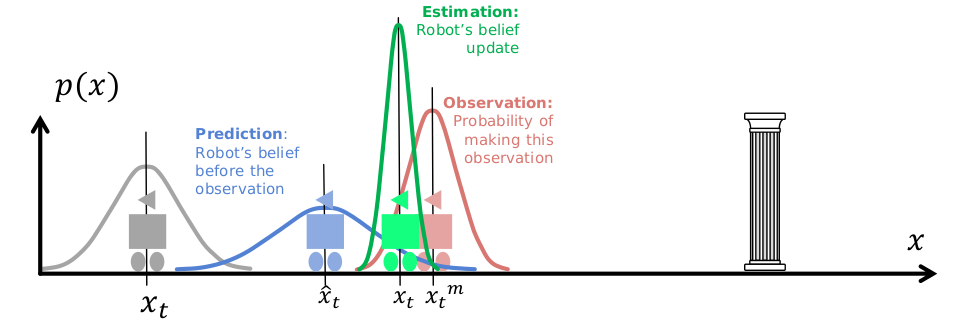
\includegraphics[width=\columnwidth]{img/9_Kalman.png}
\end{minipage}

% TODO:
% - check topological approach with Markov from book
% - performance enhancements for Markov (randomized sampling)


\vfill


\section{SLAM I}

\vmspace

\begin{minipage}{\columnwidth}
  \textit{Precedessors of SLAM:}
  \begin{compactitem}
  \item \textbf{Photogrammetry:} Use (aerial) photographs to make measurements
    between points, recover exact positions.
  \item \textbf{Structure from Motion (SfM):} Estimate 3D structure from a
    sequence of images.
  \end{compactitem}
\end{minipage}

\vpspace

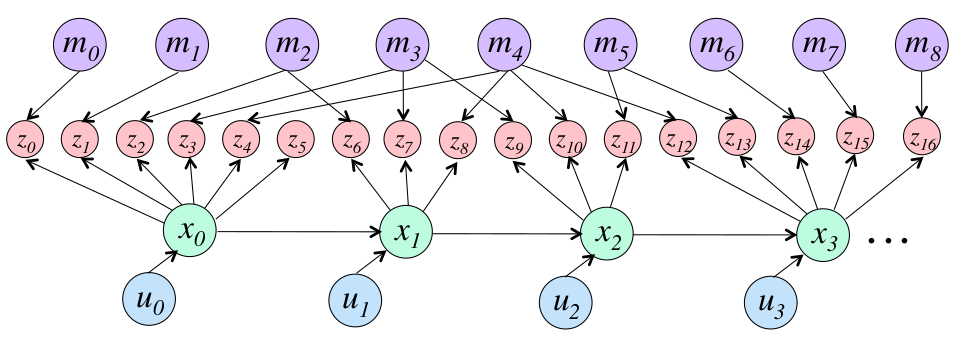
\includegraphics[width=\columnwidth]{img/10_SLAM.png}

\begin{minipage}{\columnwidth}
  \textbf{Full SLAM:} Given the the landmark observations $  \{z_0..z_k\}$ and
  the control inputs $\{u_0..u_t\}$, estimate the joint posterior
  probability over the robot path $\{x_0..x_t\}$ and the \textit{true} map
  $\{m_0..m_{n-1}\}$ , i.e. find
  \vmspace
  \begin{center}
    $
    p(x_{0:t}, m_{0:n-1}| z_{0:k}, u_{0:t}).
    $
  \end{center}
\end{minipage}

\vpspace


\begin{minipage}{\columnwidth}
  \textbf{Online SLAM:} Recover the posterior for the current pose
  \vmspace
  \begin{center}
    $
    p(x_{t}, m_{0:n-1}| z_{0:k}, u_{0:t}).
    $
  \end{center}
\end{minipage}

\begin{minipage}{\columnwidth}
  \textit{Approaches:}\\
  1) \textbf{Full graph optimization} (bundle adjustment): Eliminate
  observations and control inputs, solve for constraints between poses and
  landmarks. Sparsify graph for real-time application.
  \vspace{-17pt}
  \begin{center}
    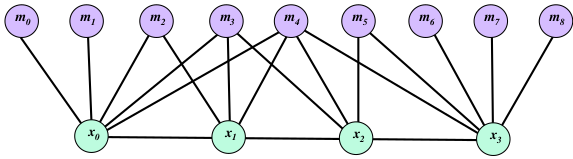
\includegraphics[width=0.5\columnwidth]{img/10_FullGraphSLAM.png}
  \end{center}
\end{minipage}

\begin{minipage}{\columnwidth}
  2) \textbf{Key frames:} Retain most representative poses and their dependency
  links, optimize resulting graph (e.g. PTAM).
  \vspace{-8pt}
  \begin{center}
    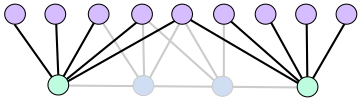
\includegraphics[width=0.5\columnwidth]{img/10_KeyframeSLAM.png}
  \end{center}
\end{minipage}

\begin{minipage}{\columnwidth}
  3) \textbf{Filtering:} Summarize all experience w.r.t. last pose with state
  vector and covariance matrix (e.g. MonoSLAM, FastSLAM).
  \vspace{-8pt}
  \begin{center}
    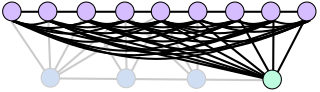
\includegraphics[width=0.5\columnwidth]{img/10_FilteringSLAM.png}
  \end{center}
\end{minipage}



\vfill


\section{SLAM II}


\begin{minipage}{\columnwidth}
  \textbf{EKF SLAM} summarizes past experience in an extended state vector $y_t$
  and a corresponding covariance $P_{y_t}$:
  \vmspace
  \begin{center}
    $
    y_t
    =
    \left[
    \begin{matrix}
      x_t \\
      m_1 \\
      \cdots \\
      m_{n-1}
    \end{matrix}
    \right],\;\;
    P_{y_t}
    =
    \left[
    \begin{matrix}
      P_{xx} & \cdots & P_{xm_{n-1}} \\
      \vdots & \ddots & \vdots \\
      P_{m_{n-1}x} & \cdots & P_{m_{n-1}m_{n-1}} \\
    \end{matrix}
    \right]
    $.
  \end{center}
  \vmspace
  S1) Prediction according to EKF equations:
  \vmspace
  \begin{center}
    $
    \hat y_t
    =
    \left[
    \begin{matrix}
      \hat x_t \\
      m_i
    \end{matrix}
    \right]
    =
    \left[
    \begin{matrix}
      f(x_{t-1}, u_t) \\
      \mathbf 0
    \end{matrix}
    \right],\;\;
    \hat P_{y_t}
    =
    F_yP_{y_{t-1}}F_y^\intercal + F_uQ_tF_u^\intercal.
    $
  \end{center}
  \vmspace
  S2) Measurement model $\hat z_i=h^i(\hat x_t, m_i)$ as in EKF localization.
  Update the state with actual observations $z_{0:n-1}$:
  \vmspace
  \begin{center}
    $
    y_t
    =
    \hat y_t + K_t v_t,\;
    P_{y_t} = \hat P_{y_t} - K_t\Sigma_{IN}K_t^\intercal$,\\
    $
    v_t=z_{0:n-1} - h_{0:n-1}(\hat x_t, m_{0:n-1}),\;
    \Sigma_{IN} = H\hat P_{y_t}H^\intercal + R,\;
    $
  \end{center}
  \vmspace
  using the Kalman gain $K_t = \hat P_{y_t}H(\Sigma_{IN})^{-1}$.
\end{minipage}

\vpspace

\begin{minipage}{\columnwidth}
  Current challenges in vision-based robotic perception:
  \begin{compactenum}
  \item High-fidelity localization and mapping.
  \item Dense scene reconstruction.
  \item Place recognition.
  \item Collaborative robot sensing and mapping.
  \item Navigation (obstacle avoidance, path planning).
  \end{compactenum}
\end{minipage}

\vfill


\section{Planning I}

\vmspace

\begin{minipage}{\columnwidth}
  \textbf{Dynamic window approach (DWA):} Acts in input space $(v,\omega)$. Set
  of admissible velocities within next time frame is
  \vmspace
  \begin{center}
    $
    V_r =
    \underbrace{V_o}_{\substack{\text{grid, obstacles} \\ \text{(in
    input-space)}}}
    \cap \underbrace{V_s}_{\substack{\text{static window} \\ \text{(motor
    limits etc.)}}}
    \cap \underbrace{V_d}_{\substack{\text{dynamic window} \\ \text{(feasible
    within next frame)}}}
    .
    $
  \end{center}
  \vmspace
  Maximize $(v,\omega)\in V_r$, subject to (local) objective function\\
  \vmspace
  \begin{minipage}{0.4\columnwidth}
    \vspace{-18pt}
    \begin{equation*}
      \begin{split}
        O =& a\cdot\mathrm{heading}(v,\omega)\\
        &+ b\cdot\mathrm{velocity}(v,\omega)\\
        &+ c\cdot \mathrm{obst\_dist}(v,\omega).
      \end{split}
    \end{equation*}
  \end{minipage}
  \begin{minipage}{0.59\columnwidth}
  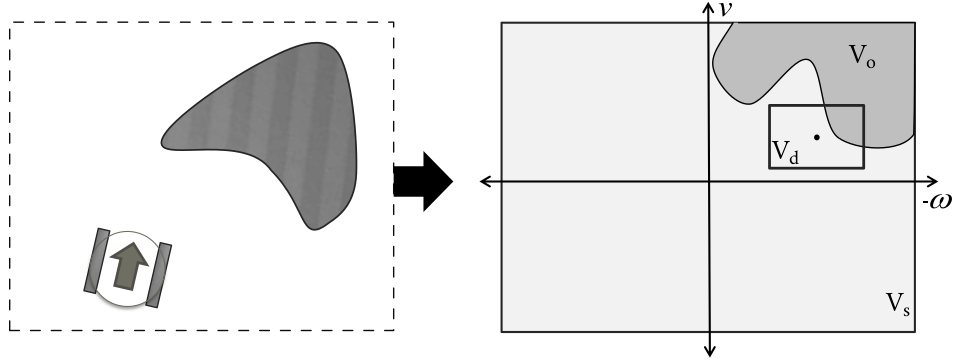
\includegraphics[width=\columnwidth]{img/12_DynamicWindow.png}
  \end{minipage}
\end{minipage}

\vpspace
\vpspace

\begin{minipage}{\columnwidth}
  \textbf{Velocity obstacles (VO):} 1) Compute set of colliding velocities. 2)
  Restrict to set of colliding velocities within time horizon $\tau$. 3) Shift
  VO by instantaneous obstacle velocity.
  \vmspace
  \begin{center}
    $
    || \mathbf p_{RO} + \mathbf v_R t || < r_R + r_O,\;\;
    \mathrm{VO}_{RO}^\tau = \bigcup\limits_{0 \le t \le \tau}
    \mathrm{Disks}\left(-\frac{\mathbf p_{RO}}{t}, \frac{r_{RO}}{t}\right).
    $
  \end{center}
  \vspace{-18pt}
  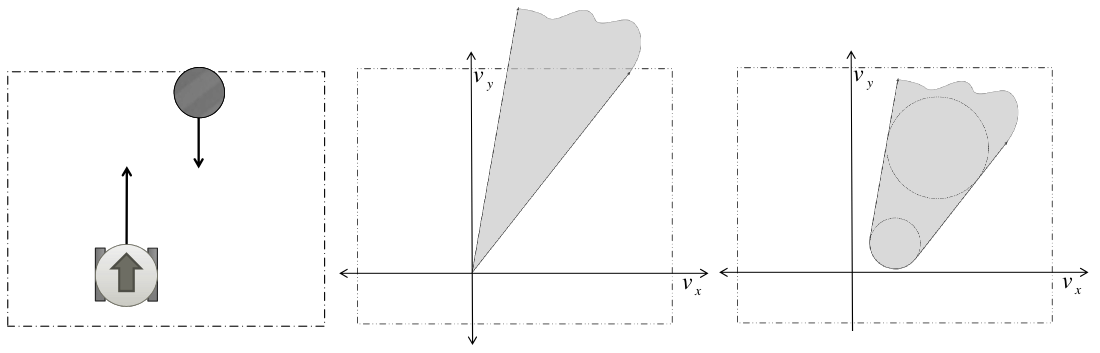
\includegraphics[width=\columnwidth]{img/12_VelocityObstacles.png}
\end{minipage}

\vpspace

\begin{minipage}{\columnwidth}
  Interactive collision avoidance for multiple decision-making agents without
  explicit communication, using a fairness property: \textbf{reciprocal velocity
  obstacles}.
\end{minipage}

\vpspace

\begin{minipage}{\columnwidth}
  \textbf{Local potential fields:} Robot (position $\mathbf q$) follows gradient
  of potential field. Potential attractive at goal, repulsive at obstacles
  ($U_\mathrm{rep} = 0$ if distance to obstacle $\rho(\mathbf q) >
  \rho_\mathrm{lim}$):
  \vmspace
  \begin{center}
    $
    U_\mathrm{att}(\mathbf q)
    =
    \frac{1}{2} k_\mathrm{att}(\mathbf q - \mathbf q_\mathrm{goal})^2,\;\;
    U_\mathrm{rep}(\mathbf q)
    =
    \frac{1}{2} k_\mathrm{rep} (\frac{1}{\rho(\mathbf q)}
    - \frac{1}{\rho_\mathrm{lim}})^2
    .
    $
  \end{center}
\end{minipage}

\vpspace

\begin{minipage}{\columnwidth}
  \textbf{Harmonic potential fields:} Iteratively solve the \textbf{Laplace
  equation}
  $
  \bigtriangleup U = \sum \frac{\partial^2 U}{\partial q_i^2} = 0
  $ with the approximation
  $
  \nabla U(\mathbf q)_i
  \approx
  [U(\mathbf q + \delta e_i) - U(\mathbf q)]/\delta
  $
  as
  \vmspace
  \begin{center}
    $
    U^{k+1}(\mathbf q)
    =
    \frac{1}{2n} \sum_{i=1}^n(U^k(\mathbf q + \delta \mathbf e_i)
    + U^k(\mathbf q - \delta \mathbf e_i)),
    $
  \end{center}
  \vmspace
  with a mixture of the following boundary conditions concerning the obstacle
  boundaries:
  \begin{compactitem}
  \item \textbf{Neumann:} Equipotential lines orthogonal.
  \item \textbf{Dirichlet:} Constant potential.
  \end{compactitem}
\end{minipage}

\vpspace

\begin{minipage}{\columnwidth}
  \textit{Additional obstacle avoidance examples:}
  \begin{compactitem}
  \item \textbf{Bug algorithm:} Follow the boundary of an obstacle, depart from
    point of shortest distance to the goal.
  \item \textbf{Vector field histogram (VFH):} Use polar histogram showing
    probability of obstacle occurence.
  \item \textbf{Bubble band technique:} Compute bubbles representing max.
    free space around given robot configuration.
  \end{compactitem}
\end{minipage}

\vfill

\vtspace

\section{Planning II}

\vmspace

\begin{minipage}{\columnwidth}
  \textbf{Road map approaches} for construction of graph $G(N,E)$ with nodes $N$
  and edges $E$:
  \begin{compactitem}
  \item \textbf{Visibility graph:} Connect nodes (obstacle corners) that
    see each other. Optimal solutions w.r.t path length.
  \item \textbf{Voronoi diagram:} Evaluate equidistant paths to obstacles,
    workspace needs to be closed.
  \end{compactitem}
\end{minipage}

\vpspace

\begin{minipage}{\columnwidth}
  General \textbf{deterministic graph search} algorithm:

  \vamspace

  \begin{algorithm}[H]
    \DontPrintSemicolon
    Queue.init(),
    Queue.push(Start)\;
    \While{\textnormal{Queue \textbf{is not} empty}}
    {
      Node curr = Queue.pop()\;
      \textbf{if} curr \textbf{is} Goal \textbf{return}\;
      Closed.push(curr)\;
      Nodes next = expand(curr)\;
      \For{\textnormal{\textbf{all} next \textbf{not in} Closed}}
      {
        Queue.push(next)\;
      }
    }
  \end{algorithm}
\end{minipage}

\begin{minipage}{\columnwidth}
  Total expected cost from start to goal via node $N$:
  \vmspace
  \begin{center}
    $f(N) = \underbrace{g(N)}_{\substack{\text{cost so far} \\
    \text{(from start)}}}
    + \varepsilon\cdot\underbrace{h(N)}_{\substack{
    \text{heuristic} \\ \text{cost-to-go}
    }
    }.$
  \end{center}
\end{minipage}

\vmspace

\begin{minipage}{\columnwidth}
  \textit{Examples:}\\
  1) \textbf{Breadth-first search}: FIFO queue, solution optimal for uniform
  edge costs, complexity: $\mathcal O (|N| + |E|)$.

  2) \textbf{Depth-first search}: LIFO queue, solution not optimal.

  2) \textbf{Dijkstra's search}: ordering according to $f(N)$ with $\varepsilon
  = 0$, complexity: $\mathcal O (|N|\log |N| + |E|)$.

  3) \textbf{A* algorithm}: extension of Dijkstra with $\varepsilon=1$. Possible
  heuristic $h(N)$: Euclidean distance to goal (underestimation).

  4) \textbf{D* algorithm}: incremental replanning version of A*.
\end{minipage}

\vpspace

\begin{minipage}{\columnwidth}
  \textbf{Binary min-heap}: Top node has minimum value.
  \begin{compactitem}
  \item \textit{Push($N$)}: Insert new node $N$ at end of heap. While $N <
    \mathrm{parent}(N)$, swap $N$ and $\mathrm{parent}(N)$.
  \item \textit{Pop()}: Return top element of heap. Move bottom node $N$ to top.
    While $N < \mathrm{min}(\mathrm{child}(N))$, swap these nodes.
  \end{compactitem}
\end{minipage}

\vpspace

\begin{minipage}{\columnwidth}
  \textbf{Rapidly exploring random tree (RRT)} algorithm as an example of a
  randomized graph search method:

  \vamspace

  \begin{algorithm}[H]
    \DontPrintSemicolon
    \SetKwFor{For}{try}{}{}
    Graph.init(Start)\;
    \While{\textnormal{Graph.size() \textbf{is less than} threshold}}
    {
      Node rand = \textbf{rand()}\;
      Node near = Graph.nearest(rand)\;
      \For{}
      {
        Node new = Sys.propagate(near, rand)\;
        Graph.addNode(new)\;
        Graph.addEdge(near, new)\;
      }
    }
  \end{algorithm}


\end{minipage}





\end{multicols}

\end{document}
